\documentclass{article}
\usepackage[utf8]{inputenc}
\usepackage{graphicx}
\usepackage{float}
\graphicspath{./}

% remove spacing around date:
\usepackage{titling}
\predate{}
\postdate{} \author{Aurelio Jethro - U1921390C}
\date{} % clear date
\title{CZ3005: TS4 - Lab II}

\begin{document}

\maketitle

\subsection*{Exercise One}
\subsubsection*{Translate the natural language statements above describing the dealing within the Smart Phone Industry in to First Order Logic (FOL)}

Constants: sumsum, appy, galactica-s3, stevey

Predicates: 
\begin{itemize}
\item Company(x) - ``x is a company''
\item Competitor(x, y) - ``x is a competitor of y''
\item Technology(x) - ``x is a smart phone technology''
\item Developed(x, y) - ``x develops y''
\item Stolen(x, y) - ``x is stolen by y''
\item Boss(x, y) - ``x is a boss of y''
\item Rival(x, y) - ``x is a rival of y''
\item Business(x) - ``x is a business''
\item Unethical(x) - ``x is unethical''
\end{itemize}

Sentence:
\begin{itemize}
\item Company(sumsum)
\item Company(appy)
\item Competitor(sumsum, appy)
\item Technology(galactica-s3)
\item Developed(sumsum, galactica-s3)
\item Stolen(galactica-s3, stevey)
\item Boss(stevey, appy)
\item $\forall$x Technology(x) $\Rightarrow$ Business(x)
\item $\forall$x, (Company(x), Competitor(x, appy)) $\Rightarrow$ Rival(x, appy)
\item $\forall$x, y, z, c (Boss(x, y) $\land$ Stolen(z, x) $\land$ Business(z) $\land$ Developed(c, z)  $\land$ Rival(c, y) $\Rightarrow$ Unethical(x))
\end{itemize}

\subsubsection*{Using Prolog, prove that Stevey is unethical. Show a trace of your proof.}

\begin{figure}[H]
    \centering
    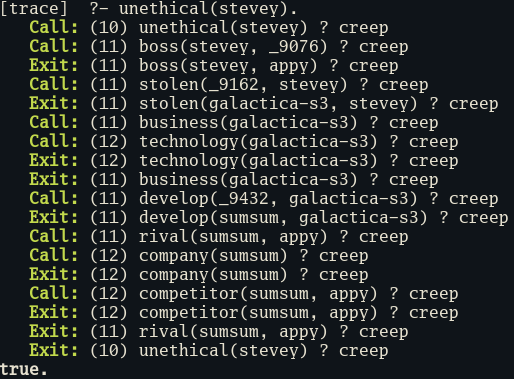
\includegraphics[width = \textwidth]{./1a.png}
\end{figure}

\subsection*{Exercise Two}

\subsubsection*{Define their relations and rules in a Prolog rule base. Hence, define the old Royal succession rule. Using this old succession rule determine the line of succession based on the information given. Do a trace to show your results.}

\begin{figure}[H]
\centering
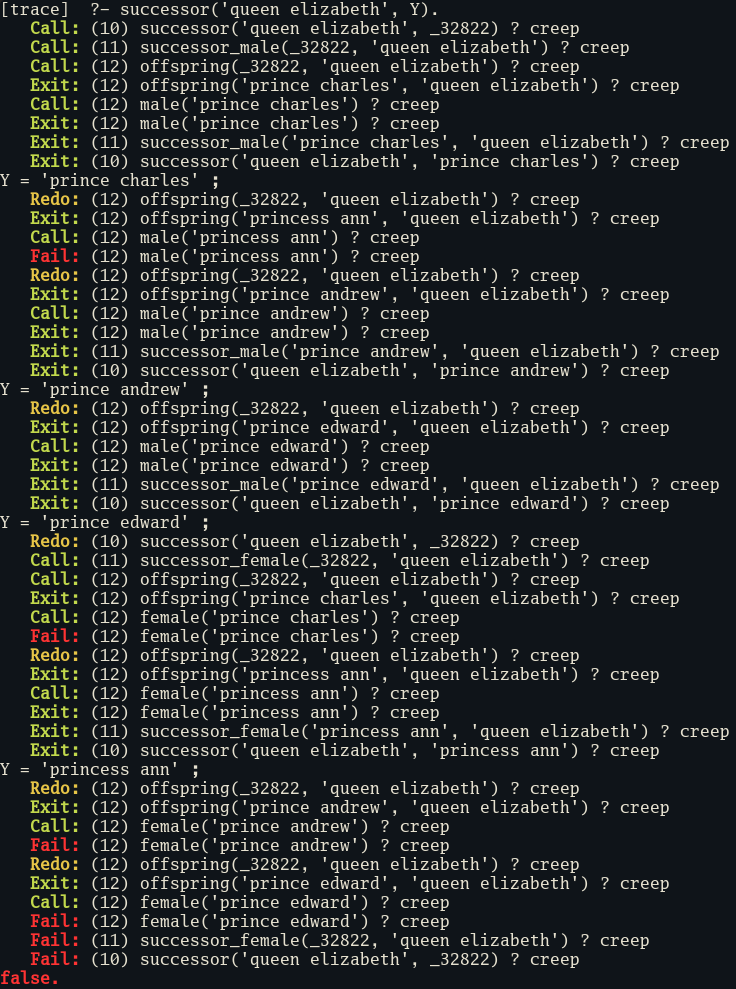
\includegraphics[width = \textwidth]{./2a.png}
\end{figure}

\subsubsection*{Recently,  the  Royal  succession  rule  has  been modified.  The  throne  is  now  passed down according  to  the  order  of  birth  irrespective  of  gender.  Modify  your  rules  and Prolog knowledge  base  to  handle  the  new  succession  rule.  Explain  the  necessary changes  to  the knowledge  needed  to represent  the  new  information.  Use  this  new succession  rule  to determine the new line of succession based on the same knowledge given. Show your results using a trace.}

\begin{figure}[H]
\centering
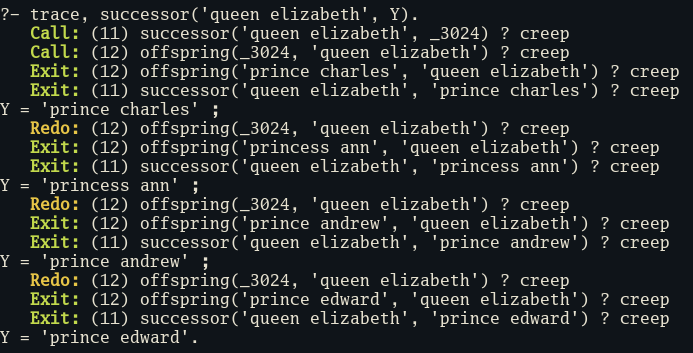
\includegraphics[width = \textwidth]{./2b.png}
\end{figure}

\end{document}
